\documentclass[border=8pt]{standalone}
\usepackage{pgfplots}
\usetikzlibrary{shapes.geometric}
\usepgfplotslibrary{groupplots}
\pgfplotsset{compat=1.18}
\renewcommand{\familydefault}{\sfdefault}
\definecolor{oursline}{HTML}{00747C}
\definecolor{omleline}{HTML}{773588}
\definecolor{uniformline}{HTML}{9D5000}
\definecolor{countline}{HTML}{2557A7}
\definecolor{ink}{HTML}{17242D}
\definecolor{muted}{HTML}{4A5C67}
\definecolor{gridline}{HTML}{E3EAED}
\begin{document}
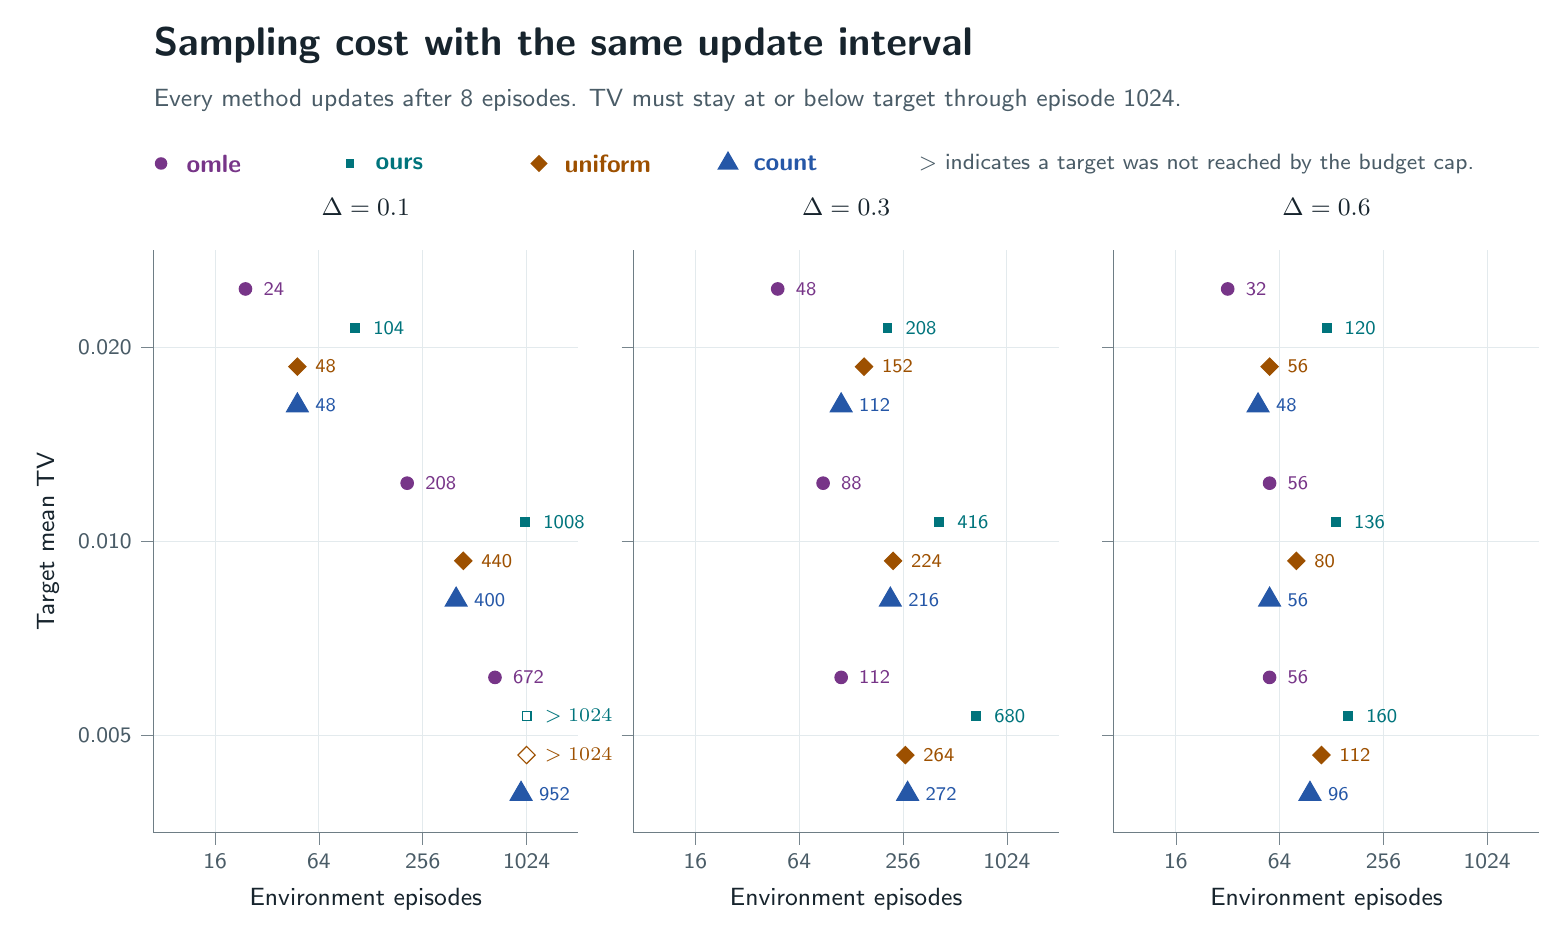
\begin{tikzpicture}[text=ink]
\begin{groupplot}[
  group style={group size=3 by 1,horizontal sep=0.7cm},
  width=5.4cm,height=7.4cm,scale only axis,
  xmode=log,log basis x=2,
  clip=false,
  tick align=outside,tick style={muted!75},
  tick label style={font=\footnotesize,text=muted},
  label style={font=\small,text=ink},
  title style={font=\small\bfseries,text=ink,yshift=1mm},
  grid=major,grid style={gridline},
  axis lines*=left,axis line style={muted!80},
  xlabel={Environment episodes},
  log ticks with fixed point,
]
\nextgroupplot[title={$\Delta=0.1$},xmin=7,xmax=2048,ymin=0,ymax=15,ytick={12.5,7.5,2.5},xtick={16,64,256,1024},xticklabels={16,64,256,1024},yticklabels={0.020,0.010,0.005},ylabel={Target mean TV}]
\node[circle,draw=omleline,fill=omleline,inner sep=1.6pt] at (axis cs:24,14) {};
\node[anchor=west,font=\scriptsize,text=omleline,xshift=3pt] at (axis cs:24,14) {24};
\node[rectangle,draw=oursline,fill=oursline,inner sep=1.6pt] at (axis cs:104,13) {};
\node[anchor=west,font=\scriptsize,text=oursline,xshift=3pt] at (axis cs:104,13) {104};
\node[diamond,draw=uniformline,fill=uniformline,inner sep=1.6pt] at (axis cs:48,12) {};
\node[anchor=west,font=\scriptsize,text=uniformline,xshift=3pt] at (axis cs:48,12) {48};
\node[regular polygon,regular polygon sides=3,draw=countline,fill=countline,inner sep=1.6pt] at (axis cs:48,11) {};
\node[anchor=west,font=\scriptsize,text=countline,xshift=3pt] at (axis cs:48,11) {48};
\node[circle,draw=omleline,fill=omleline,inner sep=1.6pt] at (axis cs:208,9) {};
\node[anchor=west,font=\scriptsize,text=omleline,xshift=3pt] at (axis cs:208,9) {208};
\node[rectangle,draw=oursline,fill=oursline,inner sep=1.6pt] at (axis cs:1008,8) {};
\node[anchor=west,font=\scriptsize,text=oursline,xshift=3pt] at (axis cs:1008,8) {1008};
\node[diamond,draw=uniformline,fill=uniformline,inner sep=1.6pt] at (axis cs:440,7) {};
\node[anchor=west,font=\scriptsize,text=uniformline,xshift=3pt] at (axis cs:440,7) {440};
\node[regular polygon,regular polygon sides=3,draw=countline,fill=countline,inner sep=1.6pt] at (axis cs:400,6) {};
\node[anchor=west,font=\scriptsize,text=countline,xshift=3pt] at (axis cs:400,6) {400};
\node[circle,draw=omleline,fill=omleline,inner sep=1.6pt] at (axis cs:672,4) {};
\node[anchor=west,font=\scriptsize,text=omleline,xshift=3pt] at (axis cs:672,4) {672};
\node[rectangle,draw=oursline,fill=white,inner sep=1.6pt] at (axis cs:1024,3) {};
\node[anchor=west,font=\scriptsize,text=oursline,xshift=3pt] at (axis cs:1024,3) {$>{}1024$};
\node[diamond,draw=uniformline,fill=white,inner sep=1.6pt] at (axis cs:1024,2) {};
\node[anchor=west,font=\scriptsize,text=uniformline,xshift=3pt] at (axis cs:1024,2) {$>{}1024$};
\node[regular polygon,regular polygon sides=3,draw=countline,fill=countline,inner sep=1.6pt] at (axis cs:952,1) {};
\node[anchor=west,font=\scriptsize,text=countline,xshift=3pt] at (axis cs:952,1) {952};
\nextgroupplot[title={$\Delta=0.3$},xmin=7,xmax=2048,ymin=0,ymax=15,ytick={12.5,7.5,2.5},xtick={16,64,256,1024},xticklabels={16,64,256,1024},yticklabels={}]
\node[circle,draw=omleline,fill=omleline,inner sep=1.6pt] at (axis cs:48,14) {};
\node[anchor=west,font=\scriptsize,text=omleline,xshift=3pt] at (axis cs:48,14) {48};
\node[rectangle,draw=oursline,fill=oursline,inner sep=1.6pt] at (axis cs:208,13) {};
\node[anchor=west,font=\scriptsize,text=oursline,xshift=3pt] at (axis cs:208,13) {208};
\node[diamond,draw=uniformline,fill=uniformline,inner sep=1.6pt] at (axis cs:152,12) {};
\node[anchor=west,font=\scriptsize,text=uniformline,xshift=3pt] at (axis cs:152,12) {152};
\node[regular polygon,regular polygon sides=3,draw=countline,fill=countline,inner sep=1.6pt] at (axis cs:112,11) {};
\node[anchor=west,font=\scriptsize,text=countline,xshift=3pt] at (axis cs:112,11) {112};
\node[circle,draw=omleline,fill=omleline,inner sep=1.6pt] at (axis cs:88,9) {};
\node[anchor=west,font=\scriptsize,text=omleline,xshift=3pt] at (axis cs:88,9) {88};
\node[rectangle,draw=oursline,fill=oursline,inner sep=1.6pt] at (axis cs:416,8) {};
\node[anchor=west,font=\scriptsize,text=oursline,xshift=3pt] at (axis cs:416,8) {416};
\node[diamond,draw=uniformline,fill=uniformline,inner sep=1.6pt] at (axis cs:224,7) {};
\node[anchor=west,font=\scriptsize,text=uniformline,xshift=3pt] at (axis cs:224,7) {224};
\node[regular polygon,regular polygon sides=3,draw=countline,fill=countline,inner sep=1.6pt] at (axis cs:216,6) {};
\node[anchor=west,font=\scriptsize,text=countline,xshift=3pt] at (axis cs:216,6) {216};
\node[circle,draw=omleline,fill=omleline,inner sep=1.6pt] at (axis cs:112,4) {};
\node[anchor=west,font=\scriptsize,text=omleline,xshift=3pt] at (axis cs:112,4) {112};
\node[rectangle,draw=oursline,fill=oursline,inner sep=1.6pt] at (axis cs:680,3) {};
\node[anchor=west,font=\scriptsize,text=oursline,xshift=3pt] at (axis cs:680,3) {680};
\node[diamond,draw=uniformline,fill=uniformline,inner sep=1.6pt] at (axis cs:264,2) {};
\node[anchor=west,font=\scriptsize,text=uniformline,xshift=3pt] at (axis cs:264,2) {264};
\node[regular polygon,regular polygon sides=3,draw=countline,fill=countline,inner sep=1.6pt] at (axis cs:272,1) {};
\node[anchor=west,font=\scriptsize,text=countline,xshift=3pt] at (axis cs:272,1) {272};
\nextgroupplot[title={$\Delta=0.6$},xmin=7,xmax=2048,ymin=0,ymax=15,ytick={12.5,7.5,2.5},xtick={16,64,256,1024},xticklabels={16,64,256,1024},yticklabels={}]
\node[circle,draw=omleline,fill=omleline,inner sep=1.6pt] at (axis cs:32,14) {};
\node[anchor=west,font=\scriptsize,text=omleline,xshift=3pt] at (axis cs:32,14) {32};
\node[rectangle,draw=oursline,fill=oursline,inner sep=1.6pt] at (axis cs:120,13) {};
\node[anchor=west,font=\scriptsize,text=oursline,xshift=3pt] at (axis cs:120,13) {120};
\node[diamond,draw=uniformline,fill=uniformline,inner sep=1.6pt] at (axis cs:56,12) {};
\node[anchor=west,font=\scriptsize,text=uniformline,xshift=3pt] at (axis cs:56,12) {56};
\node[regular polygon,regular polygon sides=3,draw=countline,fill=countline,inner sep=1.6pt] at (axis cs:48,11) {};
\node[anchor=west,font=\scriptsize,text=countline,xshift=3pt] at (axis cs:48,11) {48};
\node[circle,draw=omleline,fill=omleline,inner sep=1.6pt] at (axis cs:56,9) {};
\node[anchor=west,font=\scriptsize,text=omleline,xshift=3pt] at (axis cs:56,9) {56};
\node[rectangle,draw=oursline,fill=oursline,inner sep=1.6pt] at (axis cs:136,8) {};
\node[anchor=west,font=\scriptsize,text=oursline,xshift=3pt] at (axis cs:136,8) {136};
\node[diamond,draw=uniformline,fill=uniformline,inner sep=1.6pt] at (axis cs:80,7) {};
\node[anchor=west,font=\scriptsize,text=uniformline,xshift=3pt] at (axis cs:80,7) {80};
\node[regular polygon,regular polygon sides=3,draw=countline,fill=countline,inner sep=1.6pt] at (axis cs:56,6) {};
\node[anchor=west,font=\scriptsize,text=countline,xshift=3pt] at (axis cs:56,6) {56};
\node[circle,draw=omleline,fill=omleline,inner sep=1.6pt] at (axis cs:56,4) {};
\node[anchor=west,font=\scriptsize,text=omleline,xshift=3pt] at (axis cs:56,4) {56};
\node[rectangle,draw=oursline,fill=oursline,inner sep=1.6pt] at (axis cs:160,3) {};
\node[anchor=west,font=\scriptsize,text=oursline,xshift=3pt] at (axis cs:160,3) {160};
\node[diamond,draw=uniformline,fill=uniformline,inner sep=1.6pt] at (axis cs:112,2) {};
\node[anchor=west,font=\scriptsize,text=uniformline,xshift=3pt] at (axis cs:112,2) {112};
\node[regular polygon,regular polygon sides=3,draw=countline,fill=countline,inner sep=1.6pt] at (axis cs:96,1) {};
\node[anchor=west,font=\scriptsize,text=countline,xshift=3pt] at (axis cs:96,1) {96};
\end{groupplot}
\node[anchor=west,inner sep=0pt,font=\Large\bfseries] at ([yshift=26mm]group c1r1.north west) {Sampling cost with the same update interval};
\node[anchor=west,inner sep=0pt,text=muted,font=\small] at ([yshift=19mm]group c1r1.north west) {Every method updates after 8 episodes. TV must stay at or below target through episode 1024.};
\node[circle,fill=omleline,inner sep=1.6pt] at ([xshift=1mm,yshift=11mm]group c1r1.north west) {};
\node[anchor=west,font=\small\bfseries,text=omleline] at ([xshift=3mm,yshift=11mm]group c1r1.north west) {omle};
\node[rectangle,fill=oursline,inner sep=1.6pt] at ([xshift=25mm,yshift=11mm]group c1r1.north west) {};
\node[anchor=west,font=\small\bfseries,text=oursline] at ([xshift=27mm,yshift=11mm]group c1r1.north west) {ours};
\node[diamond,fill=uniformline,inner sep=1.6pt] at ([xshift=49mm,yshift=11mm]group c1r1.north west) {};
\node[anchor=west,font=\small\bfseries,text=uniformline] at ([xshift=51mm,yshift=11mm]group c1r1.north west) {uniform};
\node[regular polygon,regular polygon sides=3,fill=countline,inner sep=1.6pt] at ([xshift=73mm,yshift=11mm]group c1r1.north west) {};
\node[anchor=west,font=\small\bfseries,text=countline] at ([xshift=75mm,yshift=11mm]group c1r1.north west) {count};
\node[anchor=west,font=\footnotesize,text=muted] at ([xshift=96mm,yshift=11mm]group c1r1.north west) {$>$ indicates a target was not reached by the budget cap.};
\end{tikzpicture}
\end{document}
